\documentclass{standalone}

\usepackage{tikz}

\begin{document}

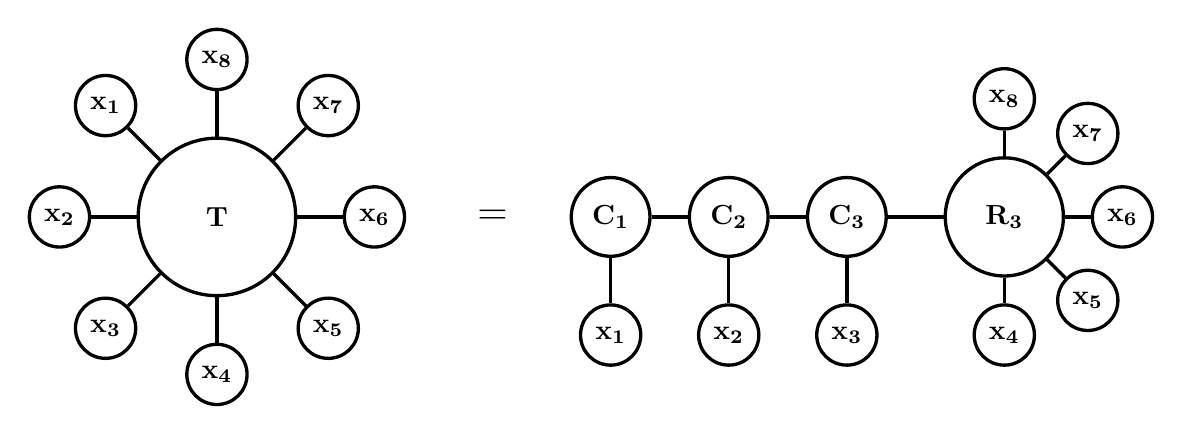
\begin{tikzpicture}[scale=1.0, every node/.style={scale=1.0}, every path/.style={line width=1.2pt}]
\node[draw, circle, line width=1.2pt, minimum size=2cm] (t) at (0,0) {$\mathbf{T}$};
\node[draw, circle, line width=1.2pt, minimum size=0.75cm] (tout1) at (0,2) {$\mathbf{x_8}$};
\node[draw, circle, line width=1.2pt, minimum size=0.75cm] (tout2) at (1.414,1.414) {$\mathbf{x_7}$};
\node[draw, circle, line width=1.2pt, minimum size=0.75cm] (tout3) at (2,0) {$\mathbf{x_6}$};
\node[draw, circle, line width=1.2pt, minimum size=0.75cm] (tout4) at (1.414,-1.414) {$\mathbf{x_5}$};
\node[draw, circle, line width=1.2pt, minimum size=0.75cm] (tout5) at (0,-2) {$\mathbf{x_4}$};
\node[draw, circle, line width=1.2pt, minimum size=0.75cm] (tout6) at (-1.414,-1.414) {$\mathbf{x_3}$};
\node[draw, circle, line width=1.2pt, minimum size=0.75cm] (tout7) at (-2,0) {$\mathbf{x_2}$};
\node[draw, circle, line width=1.2pt, minimum size=0.75cm] (tout8) at (-1.414,1.414) {$\mathbf{x_1}$};

\draw (t) -- (tout1);
\draw (t) -- (tout2);
\draw (t) -- (tout3);
\draw (t) -- (tout4);
\draw (t) -- (tout5);
\draw (t) -- (tout6);
\draw (t) -- (tout7);
\draw (t) -- (tout8);

\node (equals) at (3.5,0) {\Large $\mathbf{=}$};

\node[draw, circle, line width=1.2pt, minimum size=1.0cm] (C1) at (5,0) {$\mathbf{C_1}$};
\node[draw, circle, line width=1.2pt, minimum size=1.0cm] (C2) at (6.5,0) {$\mathbf{C_2}$};
\node[draw, circle, line width=1.2pt, minimum size=1.0cm] (C3) at (8,0) {$\mathbf{C_3}$};
\node[draw, circle, line width=1.2pt, minimum size=1.5cm] (R3) at (10,0) {$\mathbf{R_3}$};

\draw (C1) -- (C2) -- (C3) -- (R3);

\node[draw, circle, line width=1.2pt, minimum size=0.75cm] (u1) at (5,-1.5) {$\mathbf{x_1}$};
\node[draw, circle, line width=1.2pt, minimum size=0.75cm] (u2) at (6.5,-1.5) {$\mathbf{x_2}$};
\node[draw, circle, line width=1.2pt, minimum size=0.75cm] (u3) at (8,-1.5) {$\mathbf{x_3}$};
\node[draw, circle, line width=1.2pt, minimum size=0.75cm] (u4) at (10,-1.5) {$\mathbf{x_4}$};

\draw (C1) -- (u1);
\draw (C2) -- (u2);
\draw (C3) -- (u3);
\draw (R3) -- (u4);

\node[draw, circle, line width=1.2pt, minimum size=0.75cm] (u5) at (11.06,-1.06) {$\mathbf{x_5}$};
\node[draw, circle, line width=1.2pt, minimum size=0.75cm] (u6) at (11.5,0) {$\mathbf{x_6}$};
\node[draw, circle, line width=1.2pt, minimum size=0.75cm] (u7) at (11.06,1.06) {$\mathbf{x_7}$};
\node[draw, circle, line width=1.2pt, minimum size=0.75cm] (u8) at (10,1.5) {$\mathbf{x_8}$};

\draw (R3) -- (u5);
\draw (R3) -- (u6);
\draw (R3) -- (u7);
\draw (R3) -- (u8);

\end{tikzpicture}

\end{document}
